\chapter{Complexiteit}
Wanneer we code schrijven is het natuurlijk belangrijk om te weten of onze code effici\"ent is. We moeten dus met andere woorden de uitvoeringstijd kunnen vergelijken van de verschillende oplossingen van een probleem. Dit hoeft geen precieze vergelijking te zijn.  We willen een metriek die aangeeft wat de grote lijnen zijn van de performantie van een algoritme.

Een veelgebruikte manier om de complexiteit van een bepaald algoritme aan te geven is met de `big O'-notatie. In dit hoofdstuk lichten we dit concept kort toe. Volgend semester gaan jullie in het vak `toegepaste wiskunde 2' hier uitgebreider op in.

De big O-notatie  geeft aan hoe een methode zich gedraagt indien de lengte van de invoer gewijzigd wordt. Zo ga je bijvoorbeeld kunnen zien of een algoritme bij een invoer die dubbel zo groot is ook dubbel zoveel tijd gaat nodig hebben (of minder, of meer).

Als een algoritme uitgevoerd wordt, gaat de meeste tijd gespendeerd worden aan het uitvoeren van lussen in de code. Vandaar dat de big O-notatie gaat kijken naar de voorkomens van lussen in methodes, en ook gaat kijken hoe vaak door deze lussen gelopen wordt. De grootteorde van het aantal stappen dat de `zwaarste' lus uitvoert is de complexiteit van de functie.

\section{Lineaire complexiteit}

In een vorig hoofdstuk hebben we gezien hoe we een een waarde kunnen zoeken in een ongesorteerde rij. We kwamen tot deze implementatie:

\examplecode{Complexiteit/linear.js}

Dit algoritme is een voorbeeld van een algoritme met lineaire complexiteit. De big O-notatie hiervoor is: \compn. De uitvoeringstijd van dit algoritme is lineair afhankelijk met de lengte van de rij die als parameter doorgegeven wordt. Als die rij dubbel zo lang is, zal het algoritme ook dubbel zoveel tijd nodig hebben. Merk op dat ook het algoritme dat we geschreven hebben voor het lineair zoeken in een gesorteerde rij (dat gemiddeld gezien dubbel zo snel werkt) ook als complexiteit \compn heeft.

\section{Kwadratische complexiteit}

Stel dat we het aantal priemgetallen willen berekenen die kleiner of gelijk zijn dan een bepaald getal. Bijvoorbeeld, we willen weten hoeveel priemgetallen er kleiner dan 1000 zijn. We zouden deze functie kunnen schrijven als volgt:

\examplecode{Complexiteit/primes.js}

De functie krijgt een parameter n binnen die het invoergetal bevat. Ze loopt dan alle getallen af van 2 tot (n-1) in de buitenste lus. Voor elk van die getallen `i' wordt dan gekeken of dat getal een priemgetal is. Alle getallen tussen 2 en `i' worden afgegaan en er wordt gekeken of \'e\'en van die getallen een deler is van `i'. Indien geen enkel getal kan gevonden worden dat een deler is van `i', dan is `i' een priemgetal.

Het aantal keer dat de buitenste lus wordt uitgevoerd hangt lineair samen met de waarde van de parameter `n'. Als `n' dubbel zo groot is, zal de buitenste lus ook dubbel zoveel keer uitgevoerd worden. Je kan dus zeggen dat de buitenste lus O(n) stappen gaat doen. Toch is de complexiteit van dit algoritme niet O(n). Dit komt omdat \'e\'en stap van de buitenste lus uit meerdere stappen van de binnenste lus bestaat. Ook deze binnenste lus is lineair afhankelijk van de waarde van `n' (bij grotere waardes van `n' zal de binnenste lus ook meer stappen moeten uitvoeren). De binnenste lus moet dus ook O(n) stappen doen.

Elke van de \compn stappen van de buitenste lus moet dus \compn stappen doen in de binnenste lus. Het totale aantal stappen is dan \compn $\times$ \compn stappen, wat neerkomt op \compnk stappen. Dit is dan ook de totale complexiteit van het algoritme.

\section{Logaritmische complexiteit}

Zoeken in gesorteerde rijen kunnen we heel snel doen aan de hand van het binaire zoekalgoritme (zie eerder in de cursus). Herinner dat het binaire zoekalgoritme de lijst telkens in twee delen gaat verdelen en kijken in welk van de twee delen de te zoeken waarde zit. In deze deellijst wordt dan verder gezocht op dezelfde manier.

De reden waarom dit algoritme zo snel is, is omdat we in elke stap de helft van de rij kunnen uitsluiten. Als de invoer dubbel zo lang wordt, moeten we dus slechts \'e\'en stap meer doen (ten opzichte van bijvoorbeeld dubbel zoveel stappen in een algoritme met lineaire complexiteit). Dit gedrag komt overeen met de wiskundige `logaritmische' functie. Vandaar dat we zeggen dat algoritmes die dit gedrag vertonen een logaritmische complexiteit hebben, genoteerd \compln.

\section{\compnln complexiteit}

Mergesort is een algoritme dat trager is dan complexiteit \compn, maar sneller is dan complexiteit \compnk. Zoals in een eerder hoofdstuk beschreven, werkt merge sort zoals getoond wordt in Figuur~\ref{fig:mergesort}. In de eerste stap zullen de elementen in groepen van twee gezet worden en per groep gesorteerd worden. In een volgende stap worden dan telkens twee groepen samengesmolten tot \'e\'en groep. Na een aantal stappen zijn alle groepen samengesmolten tot \'e\'en grote (gesorteerde) groep.

\begin{figure}
\centering
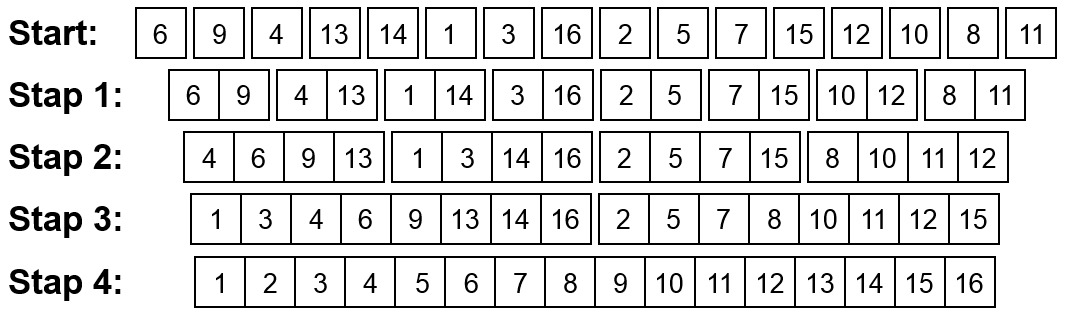
\includegraphics[scale=0.5]{Complexiteit/mergesort.png}
\caption{Schematische werking van het merge sort-algoritme}\label{fig:mergesort}
\end{figure}

Per stap zal het algoritme elk van de elementen moeten bekijken of ze op de juiste positie staan. Er moeten dus \compn vergelijkingen en verplaatsingen uitgevoerd worden. Het aantal stappen dat mergesort nodig heeft is echter ook afhankelijk van het aantal elementen in de rij. Voor n elementen zullen er $log_{2}(n)$ stappen nodig zijn (en inderdaad, $log_{2}(16) = 4$, wat overeenkomt met wat we zien in het bovenstaande voorbeeld). Als er \compln stappen nodig zijn die elk O(n) vergelijkingen en verplaatsingen doen, dan is het totaal aantal vergelijkingen/verplaatsingen gelijk aan \compln $\times$ \compn, genoteerd \compnln.

\section{Complexiteiten vergelijken}

Eenmaal de complexiteit van een algoritme gekend is, weet je of het een efficient algoritme is of niet. Voor kleine invoer (bijvoorbeeld een korte rij die gesorteerd moet worden) gaan algoritmes van verschillende complexiteiten vaak geen merkbare verschillen tonen in uitvoeringstijd, maar eenmaal de invoer groter wordt, worden de verschillen al heel snel duidelijk. Figuur~\ref{fig:complexities} toont het verloop van de complexiteiten. De horizontale as stelt de grootte van de invoer voor, terwijl de verticale as de uitvoeringstijd voorstelt. Je ziet dat de logaritmische complexiteit de beste is (van de complexiteiten die we gezien hebben). Het is een functie die snel afvlakt, en traag stijgt. Dit wil zeggen dat de invoer heel sterk moet vergroten (verdubbelen) om \'e\'en stap meer te doen. De kwadratische complexiteit stijgt het sterkst (en is dus het slechtst). Op de figuur lijkt de \compnln-complexiteit bijna even sterk te stijgen als de kwadratische complexiteit. Dit is echter `gezichtsbedrog' omwille van de kleine schaal van de grafiek. Het verloop van de \compnln is in praktijk meer vergelijkbaar met \compn dan met \compnk).

\begin{figure}
\centering
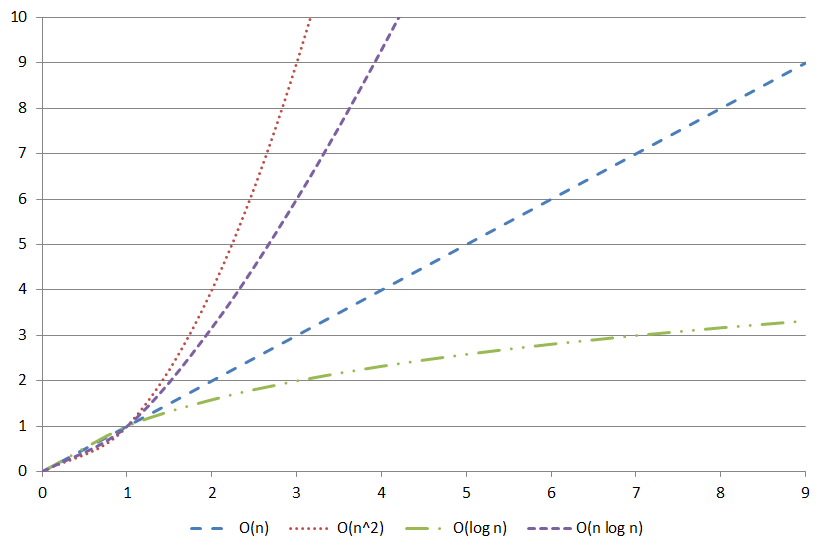
\includegraphics[scale=0.65]{Complexiteit/complexiteiten.png}
\caption{Verloop van een aantal vaak-voorkomende complexiteiten}\label{fig:complexities}
\end{figure}

Om deze grafiek een beetje tastbaarder te maken, zullen we een voorbeeldje uitwerken. Stel dat je een probleem moet oplossen (bijvoorbeeld ``zoek een element in een rij'') en dat je algoritmes hebt met verschillende complexiteiten die dit probleem kunnen oplossen. Als we er van uit gaan dat het berekenen van de oplossing voor een invoer van \'e\'en element slechts \'e\'en milliseconde duurt, dan krijgen we de resultaten in Figuur~\ref{tab:compvgl} voor een grotere invoer.

\begin{figure}
\begin{center}
\begin{tabular}{|c|c|c|c|}
\hline
& \textbf{1 element} & \textbf{1000 elementen} & \textbf{1000000 elementen} \\
\hline
\textbf{\compln} & 1 ms & 10 ms & 20 ms \\
\hline
\textbf{\compn} & 1 ms & 1 second & 16.7 minuten \\
\hline
\textbf{\compnln} & 1 ms & 10 seconden & 5.5 uur \\
\hline
\textbf{\compnk} & 1 ms & 16.7 minuten & 31.7 jaar \\
\hline
\end{tabular}
\end{center}
\caption{Vergelijking van de verschillende complexiteiten}\label{tab:compvgl}
\end{figure}

\section{Voorbeelden}

Om dit hoofdstuk af te sluiten, bespreken we nog kort de complexiteit van de sorteer- en zoekalgoritmes die we reeds gezien hebben.

\subsection{\compln}

Het binair zoekalgoritme heeft een complexiteit van \compln. In elke stap wordt het aantal elementen dat moet doorzocht worden met de helft verminderd. Dit wil zeggen dat elke keer als de lengte van de invoer verdubbelt dat het algoritme een extra stap zal moeten uitvoeren.

\subsection{\compn}

De lineaire zoekalgoritmes (zowel in een gesorteerde als niet-gesorteerde rij) hebben een complexiteit van \compn. Er is een lineair verband tussen de lengte van de invoer en de uitvoeringstijd. Dit komt omdat beide algoritmes een lus hebben die over alle elementjes van de invoer loopt. Als de invoer verdubbelt, moeten er ook dubbel zoveel stappen uitgevoerd worden.

\subsection{\compnln}

Quick sort en merge sort zijn twee voorbeelden van sorteeralgoritmes met een complexiteit van \compnln. Voor merge sort is de reden hiervoor uitgelegd in een vorige sectie in dit hoofdstuk. Quick sort heeft dezelfde complexiteit voor zeer gelijkaardige redenen. Het algoritme gaat \compln stappen doen, en in elke stap wordt de hele rij overlopen (\compn).

\subsection{\compnk}

Insertion sort, bubble sort en selection sort hebben een kwadratische complexiteit. Dit is duidelijk zichtbaar in de implementaties, die elk een lus in een lus bevatten. Beide lussen zijn afhankelijk van de grootte van de invoer, wat leidt tot een complexiteit van \compnk.

%%% Local Variables: 
%%% mode: latex
%%% TeX-master: "../main"
%%% End: 
